\documentclass{article}
\usepackage[utf8]{inputenc}
\usepackage[margin=1in]{geometry}

\title{454 - Homework 5}
\author{Victor Zhang}
\date{October 21, 2021}

\usepackage[utf8]{inputenc}
\usepackage{amsmath}
\usepackage{amsfonts}
\usepackage{natbib}
\usepackage{graphicx}
% \usepackage{changepage}
\usepackage{amssymb}
\usepackage{xfrac}
% \usepackage{bm}
% \usepackage{empheq}
\usepackage{tikz}

\newcommand{\contra}{\raisebox{\depth}{\#}}

\newenvironment{myindentpar}[1]
  {\begin{list}{}
          {
            \setlength{\leftmargin}{#1}
            \setlength{\rightmargin}{#1}
          }
          \item[]
  }
  {\end{list}}

\pagestyle{empty}

\begin{document}

\maketitle
% \begin{center}
% {\huge Econ 482 \hspace{0.5cm} HW 3}\
% {\Large \textbf{Victor Zhang}}\
% {\Large February 18, 2020}
% \end{center}

\section*{8.2}
Take a 2-by-$n$ array $X$ that satisfies the conditions. Create an ordered $2n$-tuple $A$ by putting $+ 1$ at the index of every number $x_{1j}$ in the top row and $- 1$ at the index of every number $x_{2j}$ in the bottom row. Note this tuple satisfies the Catalan condition if the array satisfies the given conditions. Namely, the partial sums $\sum_{i=0}^k A_{i}$ are nonnegative for all $k$ and in particular zero for $k = 2n$. Indeed, the condition $x_{1j} < x_{2j}$ is satisfied for all $j$ only if the partial sums never have more negative entries than positive ones, since we pair one positive entry with one negative entry in each column. Further, since we restrict the rows to be in ascending order, in fact there is a one-to-one correspondence between such tuples $A$ and arrays $X$, so we are done $\Box$

\section*{8.4a}
\tikzset{every picture/.style={line width=0.75pt}} %set default line width to 0.75pt        

\begin{center}
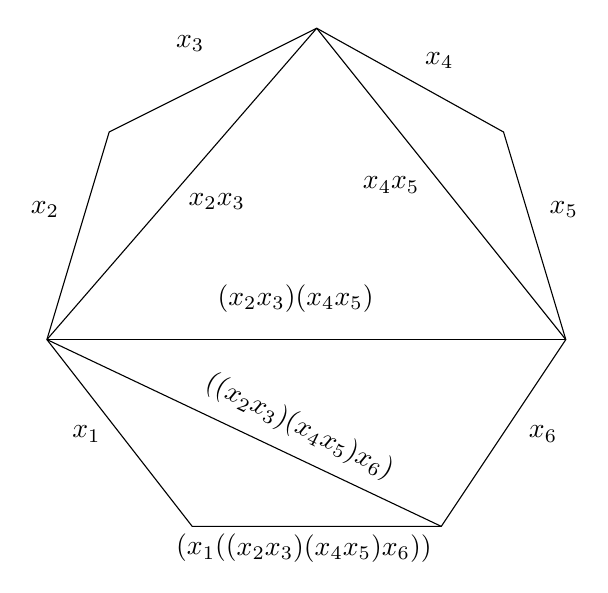
\begin{tikzpicture}[x=0.75pt,y=0.75pt,yscale=-1,xscale=1]
%uncomment if require: \path (0,341); %set diagram left start at 0, and has height of 341

%Shape: Polygon [id:ds687129078458051] 
\draw   (140,0) -- (230,50) -- (260,150) -- (200,240) -- (80,240) -- (10,150) -- (40,50) -- cycle ;
%Straight Lines [id:da11720910264541562] 
\draw    (10,150) -- (140,0) ;
%Straight Lines [id:da16032776591062148] 
\draw    (140,0) -- (260,150) ;
%Straight Lines [id:da3051016553274297] 
\draw    (10,150) -- (260,150) ;
%Straight Lines [id:da0877883329514284] 
\draw    (10,150) -- (200,240) ;

% Text Node
\draw (1,82.4) node [anchor=north west][inner sep=0.75pt]    {$x_{2}$};
% Text Node
\draw (71,2.4) node [anchor=north west][inner sep=0.75pt]    {$x_{3}$};
% Text Node
\draw (191,10.4) node [anchor=north west][inner sep=0.75pt]    {$x_{4}$};
% Text Node
\draw (251,82.4) node [anchor=north west][inner sep=0.75pt]    {$x_{5}$};
% Text Node
\draw (21,190.4) node [anchor=north west][inner sep=0.75pt]    {$x_{1}$};
% Text Node
\draw (241,190.4) node [anchor=north west][inner sep=0.75pt]    {$x_{6}$};
% Text Node
\draw (77,78.4) node [anchor=north west][inner sep=0.75pt]    {$x_{2} x_{3}$};
% Text Node
\draw (161,70.4) node [anchor=north west][inner sep=0.75pt]    {$x_{4} x_{5}$};
% Text Node
\draw (91,122.4) node [anchor=north west][inner sep=0.75pt]    {$( x_{2} x_{3})( x_{4} x_{5})$};
% Text Node
\draw (89.54,162.6) node [anchor=north west][inner sep=0.75pt]  [rotate=-26.15]  {$(( x_{2} x_{3})( x_{4} x_{5}) x_{6})$};
% Text Node
\draw (71.09,242.4) node [anchor=north west][inner sep=0.75pt]  [rotate=-0.26]  {$( x_{1}(( x_{2} x_{3})( x_{4} x_{5}) x_{6}))$};
\end{tikzpicture}
\end{center}

\section*{8.6}
\begin{center}
\begin{tabular}{|c||c|c|c|c|}
\hline
$\Delta^0$ & 3 & 4 & 9 & 18\\
\hline
$\Delta^1$ & & 1 & 5 & 9\\
\hline
$\Delta^2$ & & & 4 & 4\\
\hline
$\Delta^3$ & & & & 0\\
\hline
\end{tabular}
\end{center}
We may write $h_k = 3 \binom{k}{0} + \binom{k}{1} + 4 \binom{k}{2}$ so
$$\sum_{k=0}^n h_k = 3 \binom{n+1}{1} + \binom{n+1}{2} + 4 \binom{n+1}{3} \; \Box$$


\section*{8.19}
Recall $s(n,k)$ is the number of circular permutations of $n$ balls into $k$ nonempty bins. So $s(n,1)$ is the number of circular permutations of $n$ balls in 1 bin, or $\tfrac{n!}{n} = (n-1)!$.\\
Similarly, $s(n,n-1)$ is the number of circular permutations of $n$ balls into $n-1$ bins. This is analagous to simply picking two objects to be in the same bin and putting all the other balls into separate bins. So $s(n,n-1) = \binom{n}{2}$ $\Box$

\section*{8.26}
To calculate conjugates, we iterate over the partitions, decrementing each nonzero partition by 1. The number of decrements becomes the first partition in the conjugate, and we continue until all partitions have been decremented to zero.
\begin{gather*}
12 = 4 + 3 + 2 + 2 + 1\\
15 = 5 + 3 + 3 + 2 + 1 + 1\\
20 = 4 + 4 + 4 + 4 + 2 + 2\\
21 = 6 + 5 + 4 + 3 + 2 + 1\\
29 = 7 + 7 + 6 + 5 + 3 + 3 + 1 + 1 \; \Box
\end{gather*}


\end{document}

% List of tex snippets:
%   - tex-header (this)
%   - R      --> \mathbb{R}
%   - Z      --> \mathbb{Z}
%   - B      --> \mathcal{B}
%   - E      --> \mathcal{E}
%   - M      --> \mathcal{M}
%   - m      --> \mathfrak{m}({#1})
%   - normlp --> \norm{{#1}}_{L^{{#2}}}
